\documentclass[12pt]{article}
\usepackage{graphicx}
\usepackage{float}
\usepackage{amsmath}
\usepackage{amscd}
\usepackage{hyperref}
\usepackage{enumerate}
\usepackage{amsfonts}
\usepackage{amssymb}
\usepackage[utf8]{inputenc}
\usepackage{amsthm}
\usepackage{subcaption}
\usepackage{listings}
\usepackage{lscape}
\usepackage{tikz}
\usepackage{color} %red, green, blue, yellow, cyan, magenta, black, white
\usepackage{fullpage}
\usepackage{mathtools}
\usepackage{booktabs}
\usepackage{longtable}

\definecolor{mygreen}{RGB}{28,172,0} % color values Red, Green, Blue
\definecolor{mylilas}{RGB}{170,55,241}

\DeclarePairedDelimiter{\ceil}{\lceil}{\rceil}


\newcommand{\folder}{./Tables}
\graphicspath{{./Figuras/}}

\begin{document}


\title{Pilot 3}

\author{Instituto Tecnológico Autónomo de México}
\date{\today}
\maketitle


\hrulefill




\subsection*{Balance Table}

\begin{figure}[H]
    \caption{Cumulative number of cases by date}
    \begin{center}
        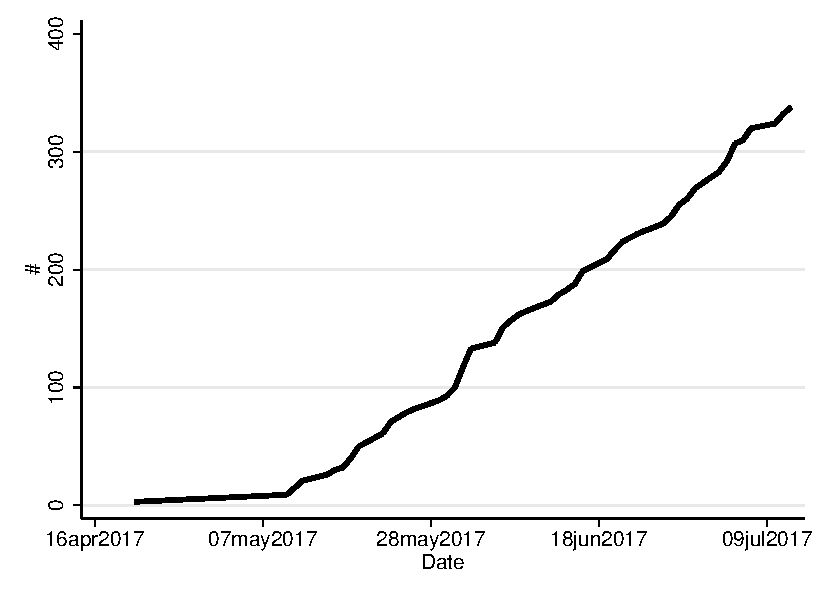
\includegraphics[width=0.7\textwidth]{cum_num_cases.pdf}
        \end{center}
    {\footnotesize \textit{Notes:Cumulative number of cases by date.}}
    {\footnotesize \textit{Do file: } \texttt{cum\_num\_cases.do}}
\end{figure}



\begin{table}[H]
\caption{Balance table}
\begin{center}
\scriptsize{% Table generated by Excel2LaTeX from sheet 'Balance'
\begin{tabular}{lccccc}
\toprule
Variable & \multicolumn{4}{c}{Treatment} & \multicolumn{1}{l}{p-value} \\
\midrule
\midrule
      & 1A    & 1B    & 2     & 3     &  \\
\midrule
Woman & 0.282 & 0.354 & 0.508 & 0.447 & 0.05 \\
Probability winning & 0.819 & 0.796 & 0.813 & 0.890 & 0.01 \\
NA probability & 0.205 & 0.438 & 0.143 & 0.156 & 0 \\
Amount Winning & 71437.500 & 40285.714 & 49642.686 & 62956.712 & 0.47 \\
NA amount & 0.590 & 0.708 & 0.532 & 0.532 & 0.15 \\
Salary & 4972.754 & 6132.651 & 4597.163 & 5581.490 & 0.41 \\
Daily Wage & 298.281 & 288.723 & 254.483 & 304.766 & 0.21 \\
Retail & 0.361 & 0.319 & 0.238 & 0.121 & 0 \\
Outsourcing* & 0.194 & 0.191 & 0.175 & 0.364 & 0 \\
Mon-Tue & 0.308 & 0.354 & 0.476 & 0.362 & 0.13 \\
+High School &       &       & 0.706 & 0.723 & 0.76 \\
Angry &       &       & 0.357 & 0.411 & 0.37 \\
Day shift &       &       & 0.857 & 0.823 & 0.45 \\
Top Sue &       &       & 0.048 & 0.064 & 0.57 \\
Big firm &       &       & 0.540 & 0.674 & 0.03 \\
Outsourcing  &       &       & 0.214 & 0.262 & 0.36 \\
At will worker &       &       & 0.071 & 0.085 & 0.68 \\
Weekly rest &       &       & 0.048 & 0.064 & 0.57 \\
Sunday bonus &       &       & 0.143 & 0.248 & 0.03 \\
Holiday &       &       & 0.262 & 0.262 & 0.99 \\
Social security &       &       & 0.286 & 0.270 & 0.77 \\
Resignation letter &       &       & 0.238 & 0.170 & 0.17 \\
Reinstatement &       &       & 0.135 & 0.149 & 0.75 \\
Number of days & 6     & 8     & 17    & 20    &  \\
\midrule
Observations & 39    & 48    & 126   & 141   &  \\
\bottomrule
\bottomrule
\end{tabular}%
}
\end{center}
 \footnotesize
\textit{Notes: Balance table on some variables. Rightmost columns shows p-value for a multivariate tests of means between different arm treatments.} 
\textit{Do file: } \texttt{balance.do}
\end{table}


\begin{table}[H]
\caption{Balance table from 2017-06-15}
\begin{center}
\scriptsize{% Table generated by Excel2LaTeX from sheet 'Balance_c'
\begin{tabular}{lccccc}
\toprule
Variable & \multicolumn{4}{c}{Treatment} & \multicolumn{1}{l}{p-value} \\
\midrule
\midrule
      & 1A    & 1B    & 2     & 3     &  \\
\midrule
Woman & 0.364 & 0.455 & 0.438 & 0.432 & 0.97 \\
Probability winning & 0.921 & 0.792 & 0.793 & 0.870 & 0.05 \\
Amount Winning & 74000.000 & 44250.000 & 63608.696 & 50939.700 & 0.81 \\
Salary & 8676.332 & 6777.818 & 4358.303 & 5893.301 & 0.2 \\
Daily Wage & 390.863 & 323.270 & 260.572 & 320.141 & 0.28 \\
Retail & 0.300 & 0.364 & 0.229 & 0.137 & 0.11 \\
Outsourcing* & 0.200 & 0.273 & 0.125 & 0.384 & 0.02 \\
Mon-Tue & 0.636 & 0.636 & 0.292 & 0.432 & 0.02 \\
+High School &       &       & 0.688 & 0.770 & 0.31 \\
Angry &       &       & 0.354 & 0.473 & 0.2 \\
Day shift &       &       & 0.875 & 0.838 & 0.58 \\
Top Sue &       &       & 0.063 & 0.041 & 0.59 \\
Big firm &       &       & 0.542 & 0.676 & 0.14 \\
Outsourcing  &       &       & 0.271 & 0.284 & 0.88 \\
At will worker &       &       & 0.083 & 0.108 & 0.66 \\
Weekly rest &       &       & 0.021 & 0.108 & 0.07 \\
Sunday bonus &       &       & 0.167 & 0.257 & 0.25 \\
Holiday &       &       & 0.188 & 0.311 & 0.13 \\
Social security &       &       & 0.229 & 0.216 & 0.87 \\
Resignation letter &       &       & 0.208 & 0.135 & 0.29 \\
Reinstatement &       &       & 0.188 & 0.149 & 0.58 \\
Attended appointment &       &       & 0.000 & 0.486 & 0 \\
Confirmed appointment &       &       & 0.000 & 0.608 & 0 \\
\midrule
Observations & 11    & 22    & 48    & 74    &  \\
\bottomrule
\bottomrule
\end{tabular}%
}
\end{center}
 \footnotesize
\textit{Notes: Balance table on some variables. Rightmost columns shows p-value for a multivariate tests of means between different arm treatments.} 
\textit{Do file: } \texttt{balance.do}
\end{table}


\end{document}